% !TeX root = ../Bachelorarbeit.tex
\chapter{Einleitung}
\label{cha:Einleitung}

\section{Hinführung}
\label{sec:hinfuhrung}\index{Hinführung}
Im Jahr 2017 alleine wurden mehr als 1,8 Milliarden browser-fähige Endgeräte weltweit verkauft.\cite{statista_absatz} Der technologische Fortschritt in Hardware und Software geben dieser großen Masse an Zugängen zum Internet eine große Vielfalt an unterschiedlichsten Applikationen, die nahezu überall auf der Welt benutzbar sind, seien es Business- oder Unterhaltungs-Applikationen, Informationsdienste oder \emph{Spiele}.\\
Auch Spiele auf mobilen Plattformen, wie Smartphones, besitzen immer mehr Grafikdetails und Leistungsanforderungen.
Dem gegenüber steht ein immer noch wachsender Markt für Spiele-Klassiker unterschiedlichster Spielekonsolen, die dem Drang nach mehr Grafikdetails und Leistungshunger aus dem Weg gehen und durch Charme mit Pixeln und Nostalgie punkten. Spiele-Klassiker wie PacMan, Tetris, Super Mario und \uvm sind auch heute noch auf vielen, teils portablen, Konsolen zu finden. Es gibt weiterhin Absatz auch für alte Plattformen wie die Atari, oder den Commodore 64. Es werden sogar Neuauflagen herausgebracht von Spielen, sowie Konsolen.\footnote{Beleg fehlt noch für Artikel zur Neuauflage!} Außerdem finden sich, durch den Fortschritt bei der Virtualisierung von Computersystemen bedingt, immer mehr Emulatoren für alte Spielekonsolen inklusive vieler Spiele im Internet.
Spiele wurden für die Pioniere des Konsolen- und Heimcomputermarktes Commodore 64 und Atari zuhauf entwickelt.\footnote{Es wurden etwa 17.000 kommerzielle Titel entwickelt.\cite{commodore64}}
Die beliebtesten Spiele waren dabei unter anderem die Folgenden:\footnote{Rankings nach Seiten X und Y}.\\
Mit dabei ist stets auch das Spiel, um das sich die Arbeit dreht: \emph{Archon}.\\
\index{Archon!Cover}
\begin{figure}[htp]
\centering
\captionsetup{justification=centering}
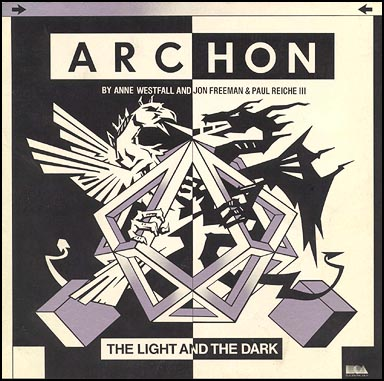
\includegraphics[width=0.50\textwidth]{Archon.jpg}
\caption[Archon - Cover]{Archon - Cover\footnotemark}
\label{fig:Archon_Cover}
\end{figure}
\footnotetext{\Quelle{C64-Wiki, \url{https://www.c64-wiki.com/wiki/Archon}}}

Spielen im Allgemeinen sind kaum noch Grenzen gesetzt. Die Spieleindustrie hat 2018 das erste Mal den Umsatz der Film- und Unterhaltungsindustrie überstiegen, sodass auch für jegliche Ideen genug Absatz und Kapital gefunden wird.\\
Plattformen für Spiele gibt es ebenfalls genügend für jeden Geschmack, ob Konsole, Computer und heutzutage auch Smartphone, Browser und sogar der Fernseher.
Die klaren Vorteile des Web als Plattform, auch für Spiele, sind dabei die Offenheit, der einfache Zugang und die immer weiter steigende Unterstützung neuer Technologien.\\
So sind heutzutage hardwarebeschleunigte 3D-Visualisierung und Echtzeitkommunikation im Webbrowser Stand der Technik.
In dieser Arbeit soll die Verschmelzung von State of the Art Webtechnologien mit einem Spieleklassiker erfolgen.\\
"Archon" genoss für Atari und C64 großen Erfolg, ähnlich vieler anderer Spiele für die Konsolen der 80er.
\todo{Anmerkung \& Recherche zu Erfolg von Archon belegen!}
Das Spiel dient daher als sehr gutes Exempel für die Möglichkeiten des Webs als Spieleplattform, aber auch der Möglichkeiten und Freiheiten des Webs für jede andere Art von Applikation.
\begin{itemize}
	\item Verkaufte Konsolen
	\item Produzierte Spiele und Verkäufe
	\item Neuauflagen von Spielen und Konsolen
	\item Neuauflagen von Archon 
	\item Virtualisierung und Emulatoren um alte Spiele zum Anfassen zu bekommen
	\item Aber, nur auf richtigen PCs zu finden und meist nicht wirklich legal
	\item Web als freie, riesige Plattform mit großem Zugriffsbereich
	\item Web APIs, die in den letzten Jahren erschienen sind (kurze Recherche zu Arbeiten des W3C!)
	\item Schiere Vielfalt an JS-Frameworks zu Web APIs und Komfort bei der Entwicklung (npm packages um Zahlen zu bekommen)
	\item Beispiele zu 3D-Möglichkeiten im Web, Stichwort: THREE.JS-Demos
\end{itemize}

\section{Aktueller Forschungsstand}
\label{sec:aktueller_forschungsstand}\index{Forschungsstand}

\emph{Hier sollen dann Extrema zum einen in Richtung 3D-Entwicklung, in Richtung Web-Entwicklung und aber auch bei der Spiele-Entwicklung kurz herausgearbeitet werden, um dem Leser einen kurzen Einblick in aktuelle Möglichkeiten zu geben, und zu zeigen, dass die Arbeit "State of the Art" ist.}
\begin{itemize}
	\item Das Web
		\subitem Viele APIs als Standard freigegeben
		\subitem Verschlüsselung immer wichtigeres Thema
		\subitem Mobile \& Offline First
		\subitem 
	\item Grafik Rendern im Browser
		\subitem Flash
		\subitem SVG, pures HTML + CSS
		\subitem Canvas
		\subitem WebGL für aufwändige 3D-Grafik (noch kein vollständiger Standard!)
	\item Games
		\subitem komplexeste Spiele sind MMO*
		\subitem Serverlose Strukturen/Nutzung von Cloud-Services
		\subitem Skalierung
		\subitem Budget
\end{itemize}

Dieses Kapitel behandelt den Einstieg in aktuelle Themen der Spieleentwicklung und des Internet. Zunächst wird dabei auf aktuell stark behandelte Themen des W3C -- dem Konsortium zur Standardisierung des Web, eingegangen. Dabei wird das Thema Grafik im Web noch einmal gesondert eingeführt. Abschließend wird auf aktuelle Probleme, Herausforderungen und Eigenschaften der heutigen Spieleindustrie eingegangen.

\paragraph{aktuelle Themen des W3C}
Das W3C hat im Moment acht Kernthemen im Rahmen Web Design und Applikationen.
Mit MathML soll ein Standard für die Anzeige von mathematischen Ausdrücken geschaffen werden. Weiterhin wird in den Themen Privacy, Accessibility, Internationalization und Mobile Web stark geforscht und an Standards gearbeitet um möglichst jedem Menschen der Welt, mit jedem internetfähigen Gerät, den vollen und sicheren Zugang zum Internet zu ermöglichen. Die in dieser Auflistung noch fehlenden Themen sind die Audio \& Video API, sowie Graphics.

Sogenannte Spiele-Engines, also Bibliotheken die sich um die meisten, generellen Problemstellungen eines Spiels und seiner Entwicklung kümmern, gibt es daher auch für browserbasierte Spiele allerlei.

\section{Motivation / Problemstellung}
\label{sec:motivation}\index{Motivation}
\emph{ Diese Sektion soll vom vorherigen Stand der Forschung und Möglichkeiten auf Anwendbarkeit überleiten und zeigen, dass die evtl. surreal erscheinende Vermischung von Genres, Plattformen und Technologien anwendbar ist, und das sogar mit beschränktem Aufwand. Vereinbarkeit von aktuellen Technologien mit Spiele-Klassikern und Spiele-Klassiker als Anwendungsbeispiele dafür.}
Bisher sind oftmals nur Demonstrationen, kurze Starter-Kits \bzw Einstiegspunkte einzelner Web-Technologien und Frameworks im Web zu finden.\\
Als Entwickler bietet es sich jedoch an auf gleiche, oder ähnliche gelöste Problemstellungen zurückgreifen zu können.
Anhand der Webapplikation sollen die Möglichkeiten des Webs dargestellt werden und weiterhin kann das Spiel als Beispiel für typische Problemstellungen eines Entwicklers für Browserspiele dienen.
Versionen, Ableger und Kopien des Spieleklassikers Archon gibt es zahlreich. Meist sind diese jedoch auf ein System beschränkt, oder tatsächlich nur mit einem Emulator ausführbar. Das Web leistet an dieser Stelle die perfekte Abhilfe: Es gibt unzählige Geräte, die heutzutage einen Webbrowser installiert haben, somit hat jeder Zugriff auf diesen Ableger, der ein webfähiges Gerät besitzt.

\section{Zentrale Begriffe}
\label{sec:zentrale_begriffe}\index{Zentrale Begriffe}

\subsection{Was versteht man unter Webtechnologien?}
Webtechnologien betiteln meist die Sammlung aller Aspekte zum Erstellen, Warten und Entwickeln einer Webanwendung.\\
Webanwendungen selbst bestehen aus einem Client-Server-Modell.
Typische Bestandteile des Clients sind: 
\begin{itemize}
	\item HTML zur Beschreibung des Inhalts
	\item CSS zur Beschreibung des Aussehens
	\item JavaScript zur Dynamisierung des Clients
\end{itemize}
Ein Webserver gibt auf HTTP-Anfragen die entsprechenden Inhalte und Medien an den Client heraus, welcher durch einen Webbrowser angezeigt wird. Außerdem können hier Daten des Clients verarbeitet, gespeichert und verteilt werden werden.
\subsection{Was versteht man unter 3D-Technologien?}
Da ein Bildschirm, beispielweise eines Computers, nur zweidimensional ist, muss durch andere Methodiken der Effekt einer dritten Dimension geschaffen werden.\\Objekte im 3D-Raum werden über ihre Eckpunkte aufgespannt und im Code somit in einem 3D-Raum mit normalem 3-Achsen-Koordinatensystem dargestellt. Anschließend folgt der Prozess des Renderns, bei dem zunächst aus den einzelnen Punkten der Objekte die Formen errechnet werden, indem die Eckpunkte zu Flächen verbunden werden. Anschließend erfolgt eine Ausrichtung aller Flächenpunkte am Pixel-Raster, sodass eine 3D-Projektion der 2D Pixel entsteht. Der nächste Schritt, Fragment-Bearbeitung, behandelt die Einfärbung der, im vorherigen Schritt gebildeten, "Fragmente" anhand von Licht und verwendeten Texturen. Der finale Schritt des Renderns wandelt die 3D-Projektion in ein 2D-Pixel-Bild, dass dann auf dem Bildschirm angezeigt wird. Außerdem werden hier Prüfungen für die Sichtbarkeit von Objekten unternommen, sodass nicht sichtbare Objekte, oder Teile von ihnen, auch nicht weiter verarbeitet werden.

\section{Ziel dieser Arbeit}
\label{sec:ziel_dieser_arbeit}\index{Ziel}
Der Schwerpunkt dieser Arbeit befasst sich mit der Umsetzung des bekannten Spieleklassikers Archon mit Web- und 3D-Technologien.
Ziel dieser Arbeit ist es eine Webapplikation zu erstellen, die den Spieleklassiker Archon in einem 3D-Stil widerspiegelt.
Die Webapplikation soll dabei folgende generelle Anforderungen erfüllen, die im Laufe dieser Arbeit näher spezifiziert werden:
\begin{itemize}
	\item Es muss mittels Webtechnologien implementiert werden
	\item Das Spiel muss in einem 3D-Stil angezeigt werden
	\item Das Spiel muss als solches wiedererkennbar sein
\end{itemize}

\section{Aufbau}
\label{sec:aufbau}\index{Aufbau}

Im ersten Teil dieser Arbeit sollen die Anforderungen an eine Neuauflage von "Archon" erfasst werden und eine Beschreibung der Features und Spielmechaniken zur Umsetzung erstellt werden.
Darauffolgend werden die Anforderungen der technologischen Seite herausgearbeitet, sodass eine Liste an Funktionalitäten entsteht, die von den 3D- und Webtechnologien erfüllt werden muss.
Anschließend wird der Aufbau der Entwicklungsumgebung, sowie benutzte Hilftmittel und getroffene Vereinfachungen beschrieben.
Alle Anforderungen werden dann in eine Beschreibung zur Umsetzung und in eine entsprechende Architektur ausgearbeitet.
Die Implementierung wird in Ausschnitten gezeigt, die die einzelnen Schritte und die Vorgehensweise bei der Umsetzung von Architektur und Programmierung aufzeigen sollen.
Den Abschluss bildet eine Überprüfung auf die Erfüllung der Anforderungen mit kurzem Einblick auf den abschließenden Stand und eine Reflexion des Ergebnisses mit Ausblick auf Folgearbeiten an der Webapplikation.